\documentclass[12pt]{article}

\usepackage{sbc-template}
\usepackage{graphicx,url}
\usepackage[utf8]{inputenc}
\usepackage{fancyhdr}
\usepackage[brazil]{babel}
%\usepackage[latin1]{inputenc}  

\pagenumbering{gobble}                          % sets page numbering off
\pagestyle{fancy}\setlength\headheight{100pt}   % set the pagestyle to fancy to include headers and footers
\pagestyle{fancy}\setlength\textheight{650pt}
\pagestyle{fancy}\setlength\footskip{20pt}
\fancyhf{}                                      % clear the header and footer
\renewcommand{\headrulewidth}{0pt}              % no horizontale ruler under header
\fancyhead[L]{
\includegraphics[width=3.8cm]{img/LogoINCT.jpg}}
\fancyhead[R]{
\includegraphics[width=3.8cm]{img/LogoOdissea.jpg}}

\begin{document} 

%\title{Guia para o carregamento de dados no Geonode Odisseia}
%\date{}
%\maketitle
%\thispagestyle{fancy}

\begin{center}
  \vspace{12pt}
  \Large\textbf{Guia para carregamento de dados no Geonode Odisseia}
\end{center}

\section{Introdução}

Este documento define procedimentos a serem utilizados no ambiente Geonode do
Odisseia para a carga de dados e a manutenção de seus estilos, metadados e
relacionamentos. O documento também traz instruções para a criação de mapas no
ambiente.

\section{Acesso} \label{sec:firstpage}

Para carregar arquivos no sistema Geonode, o usuário deve estar conectado em
uma conta com permissão para a carga. Para isso o usuário deve seguir o link na
parte superior direita da página para a tela de login e inserir suas
credenciais (Figura \ref{fig:login}).

\begin{figure}[ht]
  \centering
  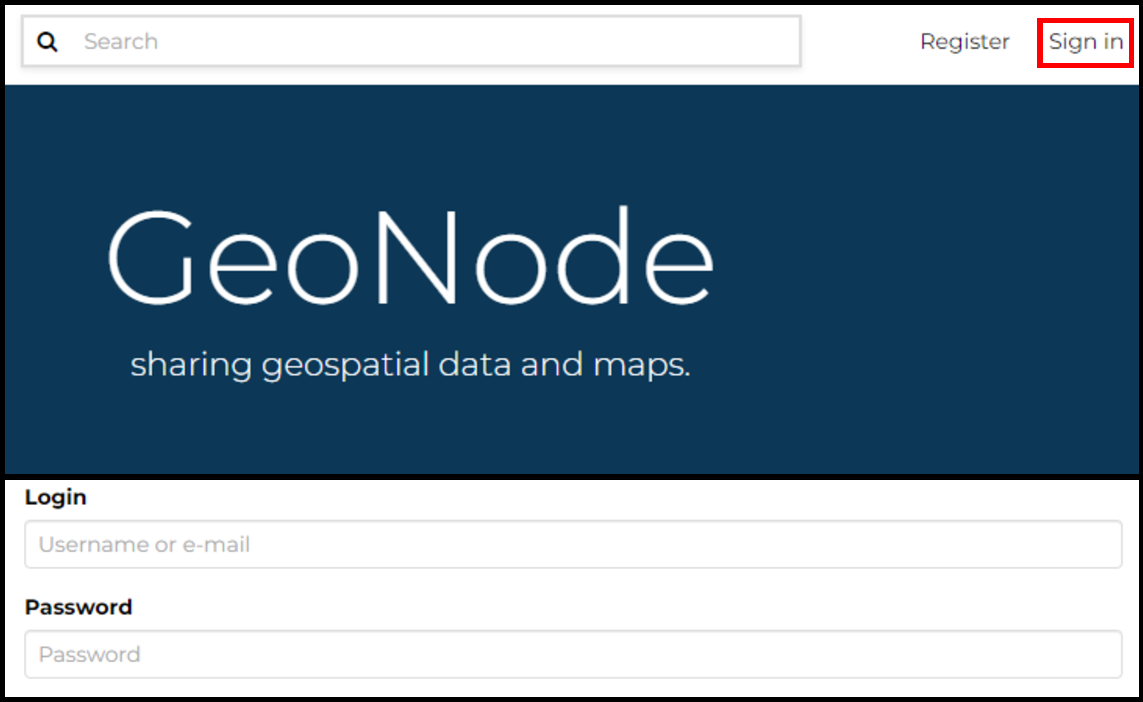
\includegraphics[width=\textwidth, keepaspectratio]{img/login.pdf}
  \caption{Caminho para a inserir as credenciais de login, em vermelho o link para acessar a página de login.}
  \label{fig:login}
\end{figure}


\section{Carga de dados e documentos}

Com o acesso ao usuário com permissões para carga será possível visualizar o
menu de "Dados" no canto superior esquerda da página (Figura
\ref{fig:upload}.1). Duas opções estão disponíveis: datasets e documentos.
Datasets se referem aos arquivos de cunho de representação geoespacial
(shapefiles, geopackages, geojson, geotiff e outros) e documentos se referem
aos demais arquivos de registro de dados (pdf, jpeg, log, csv, zip e outros).

Após acessar o menu "Dados-Datasets" ou "Dados-Documentos" será possível
carregar novos arquivos utilizando o botão "Adicionar Recurso", no canto
superior direito da página (Figura \ref{fig:upload}.2). Em uma nova página o
usuário poderá utilizar o recurso de arrastar e soltar ou o botão de selecionar
arquivos no canto esquerdo da página (Figura \ref{fig:upload}.3), é possível
carregar mais de um arquivo durante este processo. Com os arquivos devidamente
selecionados o botão de "Upload" estará disponível para prosseguir o
carregamento (Figura \ref{fig:upload}.4). 

\textbf{Atenção, no caso de shapefiles será necessário que todos os seus
componentes sejam selecionados ou que todos os componentes sejam comprimidos em
um arquivo zip.}

Ao concluir o upload o usuário será redirecionado para uma página listando
todos os arquivos carregados. Ao clicar no nome do arquivo o usuário poderá
acessar sua página de detalhamento (Figura \ref{fig:upload}.5). O mesmo pode
ser feito através do menu "Dados" acessado anteriormente, clicando na imagem de
apresentação do dado e em seguida em visualizar.

Na página de detalhamento do dado é possível visualizar, filtrar e editar os
dados geoespaciais.

\begin{figure}[ht]
  \centering
  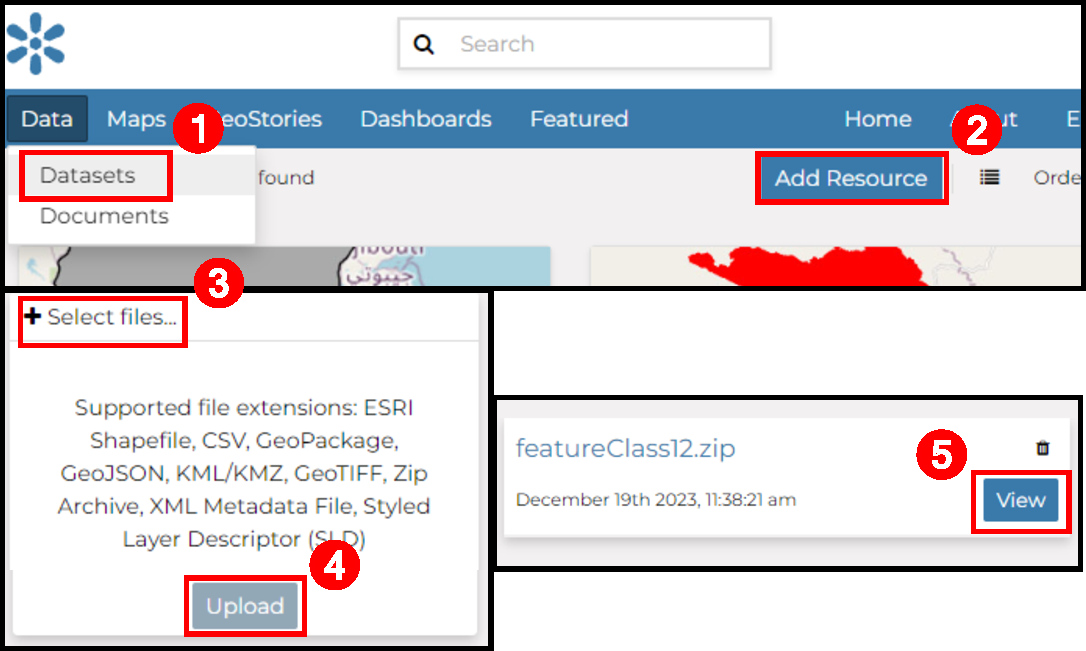
\includegraphics[width=\textwidth, keepaspectratio]{img/upload.pdf}
  \caption{Fluxo para o upload de dados no Geonode.}
  \label{fig:upload}
\end{figure}

\subsection{Estilo}

Na página de detalhamento de um dado é possível editar seu estilo através do
menu "Editar-Editar Estilo" (Figura \ref{fig:estilocodigo}.1).

O usuário pode utilizar o editor de estilo nativo do Geonode ou importar o
estilo do QGIS através de um arquivo SLD. Para importar estilos através do SLD
selecione o editor de código no canto superior direito do menu de edição de
estilo (Figura \ref{fig:estilocodigo}.2) e insira o texto de descrição SLD
criado pelo QGIS (Figura \ref{fig:estilocodigo}.3). Por fim aplique as
alterações (Figura \ref{fig:estilocodigo}.4).

\begin{figure}[ht]
  \centering
  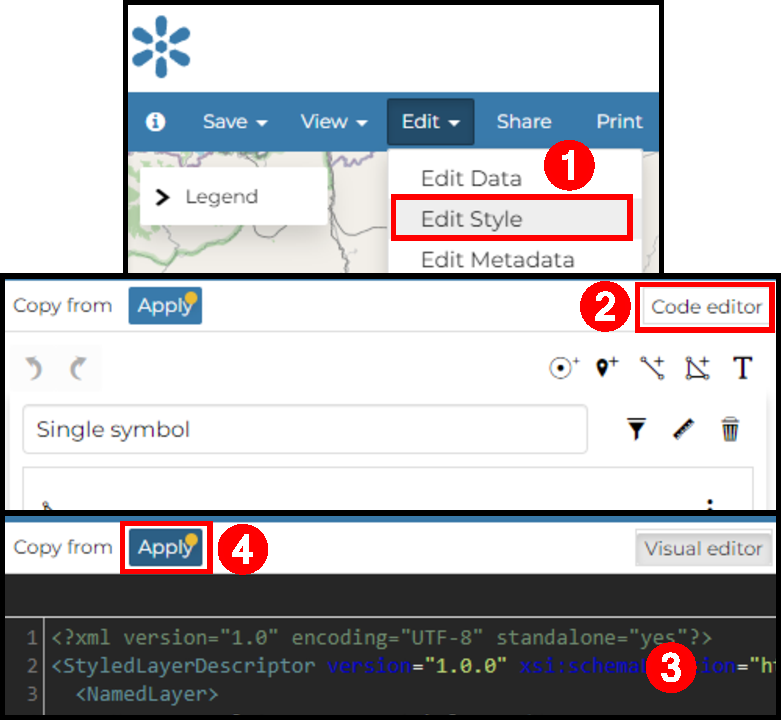
\includegraphics[width=\textwidth, keepaspectratio]{img/estilocodigo.pdf}
  \caption{Fluxo para a importação de estilo de um arquivo SLD.}
  \label{fig:estilocodigo}
\end{figure}

\subsubsection{Criando estilos SLD no QGIS}

No QGIS, na lista de camadas, clique com o botão direito na camada que deseja
exportar o estilo em SLD (Figura \ref{fig:exportarsld}.1). Siga para o menu
"Propriedades" e "Simbologia". No canto inferior esquerdo do menu simbologia
clique em "Estilo" e em seguida em "Salvar estilo" (Figura
\ref{fig:exportarsld}.2). No novo menu selecione o estilo SLD (Figura
\ref{fig:exportarsld}.3) e salve em um local a sua escolha.

\begin{figure}[ht]
  \centering
  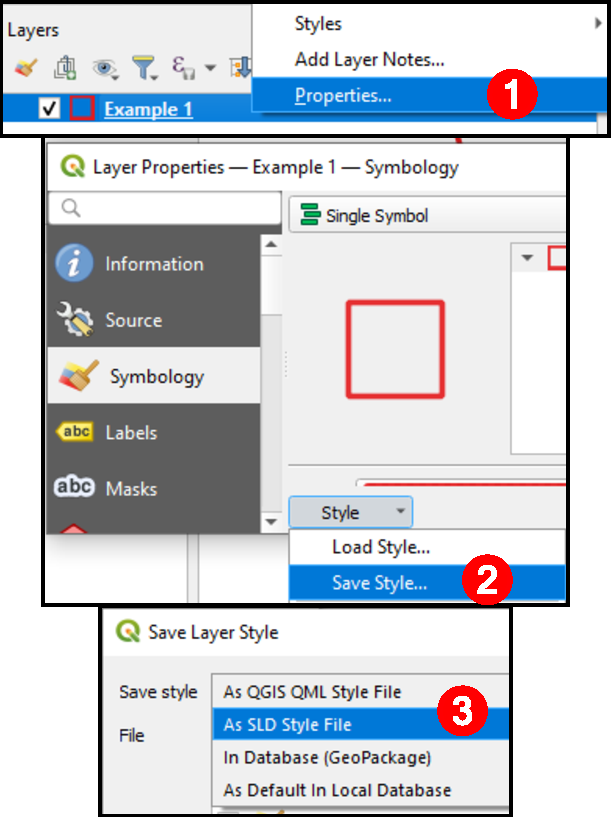
\includegraphics[width=10cm, keepaspectratio]{img/exportarsld.pdf}
  \caption{Fluxo para a exportação de um estilo para um arquivo SLD.}
  \label{fig:exportarsld}
\end{figure}

\subsection{Metadados}

Na página de detalhamento de um dado é possível editar seus metadados através
do menu "Editar-Editar Metadados" (Figura \ref{fig:metadado}.1). 

Na página de edição de metadados o usuário pode alterar todos os aspectos do
metadado através de um formulário (Figura \ref{fig:metadado}.2). A medida que
os campos são preenchidos uma barra de progresso é atualizada (Figura
\ref{fig:metadado}.3), quando completa o metadado possui informações
suficientes para cumprir com os requisitos da iso 19.115.

\begin{figure}[ht]
  \centering
  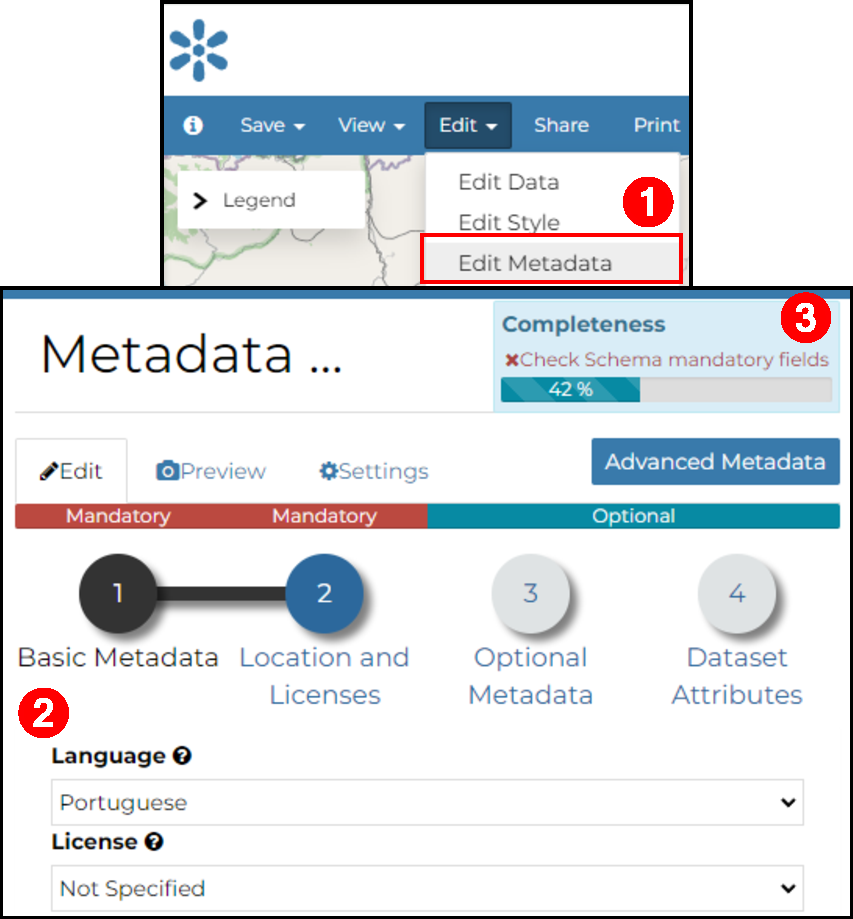
\includegraphics[width=10cm, keepaspectratio]{img/metadado.pdf}
  \caption{Acesso, edição e progresso de um metadado.}
  \label{fig:metadado}
\end{figure}

Grande parte das informações necessárias para a formação do metadado são
extraídas automaticamente do dataset pelo Geonode. Os dados que requerem
inserção manual para um metadado completo são:

\begin{itemize}
  \item Título
  \item Abstract
  \item Data de publicação/criação
  \item Categoria
  \item Palavra-chave
  \item Idioma
  \item Licença
  \item Atribuição
  \item Declaração de qualidade dos dados
  \item Restrições de uso/acesso
\end{itemize}

\textbf{Para a filtragem dos dados é importante que os metadados
 estejam preenchidos corretamente. Sendo assim, todo dado inserido deve conter
 seu sítio de pesquisa como Palavra-chave e pertencer ao grupo de seu sítio.}

\subsubsection{Relacionamento de datasets e documentos}

O relacionamento de dados permite que o usuário encontre outros dados ou
documentos que tenham correlação com o dado que esta sendo visualizado. Para
isso, é necessário definir seus relacionamentos em seus metadados. Durante a
edição de metadados, na aba de "Metadados Opcionais" (Figura
\ref{fig:relacionamentos}.1) é possível inserir "Recursos Relacionados" (Figura
\ref{fig:relacionamentos}.2). O Geonode irá listar todos os recursos
disponíveis que podem ser filtrados pela caixa de texto.

Quando um dos recursos possuir a relação, será possível seguir para o outro por
meio da aba "Recursos Relacionados" no menu à direita na tela de visualização
do dado (Figura \ref{fig:relacionamentos}.3).

\begin{figure}[ht]
  \centering
  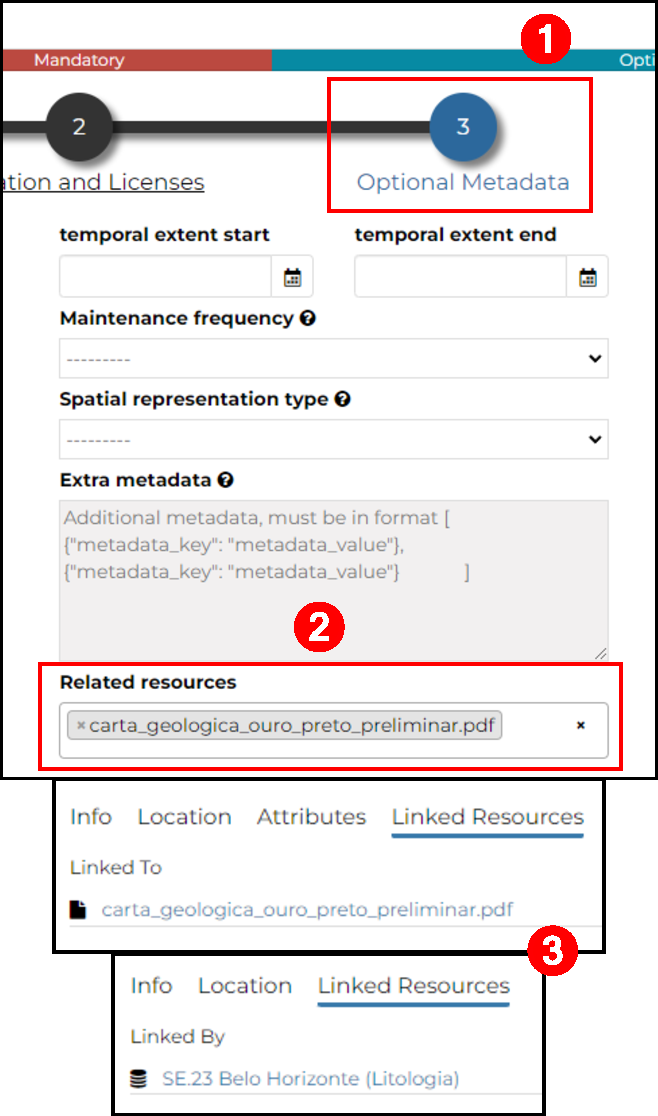
\includegraphics[width=8cm, keepaspectratio]{img/relacionamentos.pdf}
  \caption{Adicionando e visualizando relacionamentos de dados.}
  \label{fig:relacionamentos}
\end{figure}

\section{Mapas}

No menu Mapas na aba superior da página do Geonode é possível consultar os
mapas existentes e criar novos mapas (Figura \ref{fig:criarmapa}.1). Usando o
botão "Adicionar recursos" na parte superior direita da página e em seguida
"Criar mapa" (Figura \ref{fig:criarmapa}.2) é possível criar um mapa a partir
dos datasets inseridos no Geonode.

Na página do mapa utilize o botão "Adicionar dataset" no menu superior (Figura
\ref{fig:criarmapa}.3), este irá criar um catálogo a direita no qual poderão
ser adicionados os datasets ao mapa (Figura \ref{fig:criarmapa}.4). As camadas
podem ser organizadas utilizando o botão de camadas na parte superior direita
do visualizador (Figura \ref{fig:criarmapa}.5) e utilizando a ferramente de
arrastar e organizar o usuário poderá mudar a ordem de renderização dos dados
(Figura \ref{fig:criarmapa}.6).

\begin{figure}[ht]
  \centering
  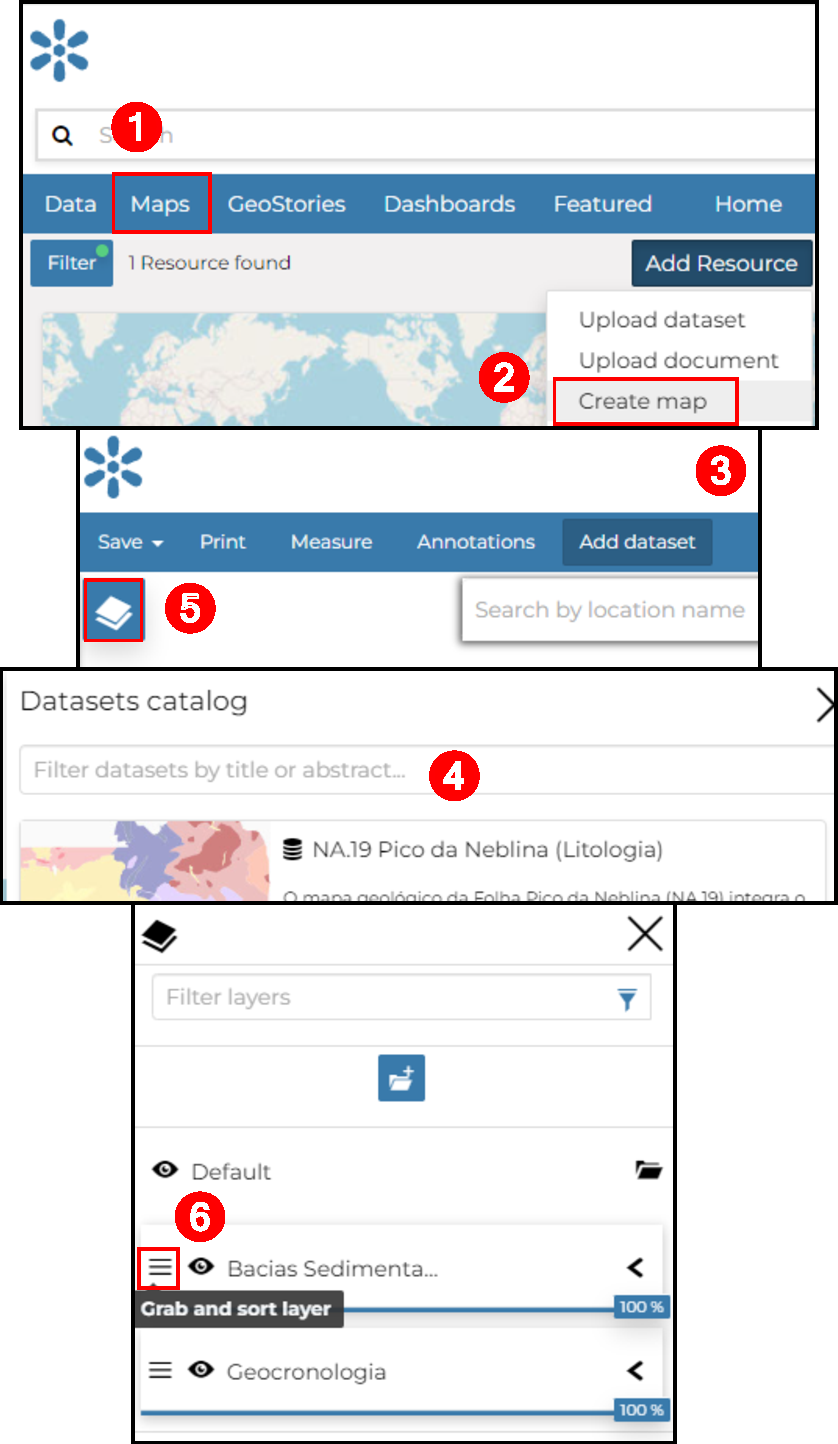
\includegraphics[width=10cm, keepaspectratio]{img/criarmapa.pdf}
  \caption{Fluxo para a criação de mapas e organização de suas camadas.}
  \label{fig:criarmapa}
\end{figure}

\bibliographystyle{sbc}
\bibliography{sbc-template}

\end{document}
